The main contribution of this work is an environment modeling a single-family household, consisting of a Rooftop Solar Array (RSA), an Energy Storage System (ESS), a Thermostatically Controlled Load (TCL), and Flexible Demand Response (FDR). The environment is a mixture of replayed data and dynamic components. It is built on the Gymnasium framework \cite{Towers.2023} and available on GitHub\footnote{https://github.com/TimWalter/smart-energy-controller}. The main objective is minimizing the CO2eq emissions. The task is split into week-long episodes with hourly resolution, to capture daily and weekly patterns of demand and generation.
\par
The RL paradigm requires the formulation as a Markov Decision Process, consisting of a transition function, action and observation spaces, and a reward function. The transition function is given by the replayed data and the dynamics of the components in the following. The observation space is a bounded subset of $\mathbb{R}^{11+H}$, with the observables given in \cref{tab:observation_space}. The action space is summarized in  \cref{tab:action_space}. The reward function is described in \cref{ssec:reward_function}.

\subsection{Replayed Data}\label{ssec:static_components}
The data was either initially given in hourly resolution or down-sampled by averaging. The most relevant observables are displayed exemplary in \cref{fig:static_components}.
\par
The auxiliary information included weather and time data, which provided means for the agent to predict the carbon intensity of the electricity mix and the heating demand. It was sourced from the Photovoltaic Geographical Information System (PVGIS) \cite{ThomasHuld.2012}.
\par
The RSA was simulated using the PVLIB library \cite{F.Holmgren.2018}, with panel specifications from the CEC database \cite{Dobos.2012}\cite{Boyson.2007}.
\par
The household's energy demand was sourced from the UCI archive \cite{GeorgesHebrail.2006}. Since the consumption was unraveled for different rooms, the kitchen, electric water heater and air conditioner were modeled as inflexible demand, while the laundry room as flexible demand.
\par
The direct carbon intensity of the electricity mix at any given time was sourced from Electricity Maps \cite{ElectricityMaps.2023}. 
\begin{figure}[H]
    \centering
    \setlength{\abovecaptionskip}{0pt}
    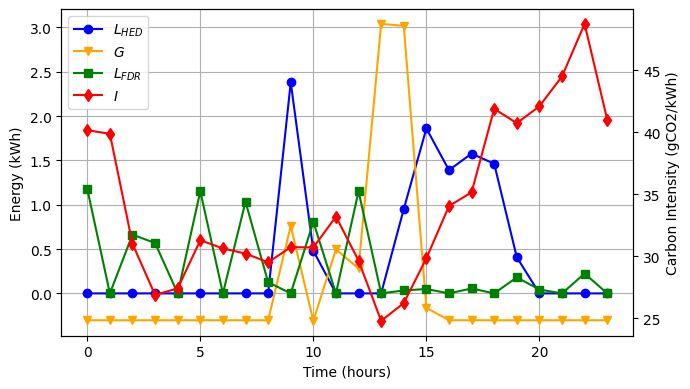
\includegraphics[width=0.45\textwidth]{figures/static_components.png}
    \caption{Replayed data for the first 24 hours.}
    \label{fig:static_components}
\end{figure}

\subsection{Energy Storage System}
The ESS is connected to the grid and the RSA. The charge is subject to the following dynamics
\begin{equation}
    B_t = \max\{0, B_{t-1} - D_s + C_t \sqrt{\nu} - \frac{D_t}{\sqrt{\nu}}\}.
\end{equation}
Here, $B_t \in [0, B_{max}]$ is the charge at time $t$ and $B_{max}$ is the capacity. Furthermore, $\nu$ denotes the round trip efficiency, $D_s$ the self-discharge rate, $C_t \in [0, C_{max}]$ the charge rate with maximum $C_{max}$, and $D_t \in [0, D_{max}]$ the discharge rate with its respective maximum $D_{max}$. 

\subsection{Flexible Demand Response}
The FDR can be influenced stochastically in a running time window of length $H$ by a signal $a_{fdr, t} \in [-1 , 1]^H$. Whether the power is consumed is determined by a Bernoulli process, with probabilities
\begin{equation}
    p_t = \text{clip}\left(s + a_{fdr, t} * \exp\left(\frac{-1}{\beta}\left|t - t_{s}\right|\right), 0, 1\right),
\end{equation}
where $s \in \{0,1\}^{H}$ indicates the desired consumption with elements $s_i = \begin{cases}
    1 & \text{if } t_i \leq t \\
    0 & \text{else}
\end{cases}$, $\beta$ is a patience parameter, and $t_{s} \in \mathbb{R}^{H}$ is the desired consumption time. If consumption is delayed more than once, $\frac{2}{H-1}$ of the power is consumed in each time step to ensure that all power has been consumed after the time window. This aims to facilitate learning by preventing infinite delays or a large correction at episode termination.

\subsection{Thermostatically Controlled Load}\label{ssec:tcl}
The TCL encapsulates all devices that aim to maintain the temperature of a given heat mass. To utilize such loads as energy storage, the temperature of the heat mass is allowed to fluctuate within a given range. The TCL is modeled as a second-order system \cite{Sonderegger.1978} with the following dynamics:
\begin{equation}
    \begin{split}
        T_t &= T_{t-1} + \frac{1}{r_a} (T_{a, t} - T_{t-1}) \\
        &+ \frac{1}{r_b} (T_{b,t} - T_{t-1}) \\
        &+ \frac{1}{r_h} L_{TCL} a_{tcl,t} + q,
    \end{split}
\end{equation}
where $T_t$ is the indoor temperature at time $t$, $r_a$ is the thermal mass of the air, $T_{a, t}$ is the current outdoor temperature, $r_b$ is the thermal mass of the building material, and $T_{b, t}$ is the current building mass temperature, that evolves with
\begin{equation}
    T_{b, t} = T_{b, t-1} + \frac{1}{r_b} (T_{t-1} - T_{b, t-1}),
\end{equation}
$\frac{1}{r_h}$ is the power-to-heat coefficient, $L_{TCL}$ is the nominal power, 
$a_{tcl_t} \in [-1, 1]$ is the heating signal, and $q$ is the unintended heat drift. The heating signal is constrained by the desired temperature range, enforced through a backup controller as follows:
\begin{equation}
    a_{tcl, t} = \begin{cases}
        -1 & \text{if } T_t \geq T_{max} \\
        1 & \text{if } T_t \leq T_{min} \\
        a_{tcl, t} & \text{else,} 
    \end{cases}
\end{equation}
where $T_{max}$ and $T_{min}$ define the desired temperature range. 

\begin{table}
\caption{Observation Space.}
\label{tab:observation_space}
\vskip 0.15in
\begin{center}
\begin{small}
\begin{sc}
\begin{tabular}{lcr}
\toprule
Observable & Symbol & Replayed\\
\midrule
Carbon Intensity & $I$ & X\\
    Household Energy Demand & $L_{HED}$ & X\\
    Rooftop Solar Generation & $G$ & X\\
    ESS Charge & $B$ & \\
    FDR power in window & $L_{FDR}$ &\\
    Indoor temperature & $T$ & \\
    Time step & $t$ & X\\
    Month of Year & $MoY$ & X \\
    Solar Irradiation & $SI$ & X\\
    Solar Elevation & $SE$ & X\\
    Outdoor temperature & $T_a$ & X \\
    Wind Speed & $WS$ & X\\
\bottomrule
\end{tabular}
\end{sc}
\end{small}
\end{center}
\vskip -0.1in
\end{table}

\begin{table}
\caption{Action Space.}
\label{tab:action_space}
\vskip 0.15in
\begin{center}
\begin{small}
\begin{sc}
\begin{tabular}{lcr}
\toprule
Action & Min. Meaning & Max. Meaning\\
\midrule
$a_{ess}$ & Discharge & Charge \\ 
    $a_{fdr}$ & Delay     & Expedite \\
    $a_{tcl}$ & Cooling   & Heating\\
\bottomrule
\end{tabular}
\end{sc}
\end{small}
\end{center}
\vskip -0.1in
\end{table}

\subsection{Reward Function} \label{ssec:reward_function}
The given objective of minimizing CO2eq emissions is augmented by a temperature discomfort penalty to bias towards the desired temperature.
%avoid unintended exploitation of the TCL, which is otherwise optimally controlled by the backup controller, once the outdoor temperature is outside the boundaries. 
The resulting reward function is
\begin{flalign}
    r_t &= I_t (E_p - E_c) - DC && \\
    \begin{split}
        E_c &= L_t + \frac{1}{r_h} L_{TCL} a_{tcl,t} + C_t \\
        &+ \sum_{p \in U_e} p_r + \sum_{p \in U_d} \frac{2p}{H-1}
    \end{split} && \\
    E_p &= G_t + D_t  && \\
    DC &= \delta \exp(|T_t - \frac{T_{max} + T_{min}}{2}), &&
\end{flalign}
where $U_e$ is the set of consumed FDR, $p_r$ is the remaining power after discounting, $U_d$ is the set of delayed FDR, and $\delta$ the discomfort coefficient. 
\par
Given that the task formulation is episodic, it differs from the real-world problem which has an infinite horizon. In the real-world problem, the initial state of the upcoming week is influenced by the past week. Therefore, to accurately reflect this, a correction is required at termination to evaluate the remaining state. The terminal reward is corrected by
\begin{flalign}
    reward &\mathrel{+}= I_t B_t && \\
    reward &\mathrel{+}= I_t (- \sum_{p \in U} p_r) && \\
    reward &\mathrel{+}= I_t (- r_h\left|T_t - \frac{T_{max}+T_{min}}{2}\right|) && 
\end{flalign}
where $U$ is the set of remaining FDR.